\documentclass[oribibl]{llncs2e/llncs}
\usepackage{geometry}                % See geometry.pdf to learn the layout options. There are lots.
\geometry{letterpaper}                   % ... or a4paper or a5paper or ... 
%\geometry{landscape}                % Activate for for rotated page geometry
%\usepackage[parfill]{parskip}    % Activate to begin paragraphs with an empty line rather than an indent
\usepackage{amssymb,amsmath}
\usepackage{graphicx}
\usepackage{amssymb}
\usepackage{epstopdf}
\DeclareGraphicsRule{.tif}{png}{.png}{`convert #1 `dirname #1`/`basename #1 .tif`.png}

\graphicspath{{WarpTask/figures/}{Res/figures/}} %do not forget the / at the end
%\include{{llncs2e}}

\title{Large integer arithmetic and polynomial inner product}
\author{Timoth\'ee Ewart\inst{1}, Andreas Hein$^2$, Matthias Troyer\inst{2} and Thierry Giamarchi\inst{1}}

\institute{Universit\'e de Gen\`eve, \email{timothee.ewart@gmail.com} \thanks{Thank you : Maxim Milakov, Peter Messmer  - NVIDIA, and  Williams Sawyer, Gilles Fourestey - CSCS}  \and Eidgen\"ossische Technische Hochschule Z\"urich }

%\date{}                                           % Activate to display a given date or no dater
\begin{document}
\maketitle
%\section{}
%\subsection{}


The main purpose of the VLI lib is performed large integer arithmetic based on meta-programming and  hybrid (CPU/GPU) inner product of polynomial up to order 14 with 1 to 4 variables with large integer coefficient 128 to 256 bits.  We remember the basics of the inner product of a polynomial,  and the implementation of the large integer library for the cpu version  The second part will be on the gpu implementation of the inner product.  All these algorithms are based on brut force attacks, as their size should not justify a FFT approach \cite{Emeliyanenko:2009}.

\section{Art of work}

BLABLABLALBALBALBLALBALBLALBLALBLALBLALBABLALB ALBLALBALBLABLALBLABLALBLA......

\section{Polynomial and Inner product definitions}

The library performed inner product of vector of polynomials from one to four variables where polynomials are defined like (four variables) :
\begin{eqnarray}
P_a(x,y,z,w) & = & \sum_i^n \sum_j^n  \sum_k^n \sum_l^n  a_{ijkl} x^i y^j z^k w^l , \,\,\,\,\,\, \text{or} \\
                   & = & \sum_i^n \sum_j^{(n-i)} \sum_k^{(n-i-j)} \sum_l^{(n-i-j-k)}  a_{ijkl} x^i y^j z^k w^l  .
\end{eqnarray}
where  $x,\,y,\,z$ and $w$ are the variables,  $i,\,j,\,k$ and $l$  the indices, $a$  the coefficients, and $n$ the order of the polynomial.
We name these polynomials max order each and max order combined, respectively.  If now we consider 2 vectors of polynomials of the  same type of $m$ 
entries  $\boldsymbol{v}_1<P_a>$ and  $\boldsymbol{v}_2<P_b>$. The inner product  consists of the product 
of every entries  associated to a global reduction. 
 
 \begin{eqnarray}
 P_c = \sum_i^m \boldsymbol{v}_{1_i}<P_a>  \times  \boldsymbol{v}_{2_i}<P_b> \label{poly1}
\end{eqnarray}

where $\times$ indicates the multiplication between two polynomials. The multiplications occurs basic rules of polynomials multiplication. We note 
a result coefficient may be not unique. It can be the sum of several coefficients resulting from the sum of several multiplications (contributions). These coefficients are named cross term. 
These cross terms are not a problem for the cpu version but they are  the bottleneck for the gpu version. 
In term of  programming and parallelization,  for the cpu version the equation  \ref{poly1} can be reduced by a basic loop with a final reduction. These work can be easily done in OpenMP. Every OpenMP threads
calculate several  polynomial multiplications and make a local reduction. At the end, a final reduction is performed  by the main thread \footnote{In OpenMP reduction for class is not supported}. 

\section{VLI  CPU library}

The coefficients of the polynomial are represented by a large integer named VLI number.  A VLI number is characterized by is Size in bits; it is a  template parameter.
The size varies from 128 to 512 buts.  Its implementation is static, contrary to the well know GMP \footnote{gmplib.org} and determined during the compilation time. 
Inside the memory, the VLI numbers are  contiguous. The data type container is an 64 bits unsigned integer

The basic operations supported by VLI are the four basic operations : $+,-,\times, /$, extended multiplication and bit shift operations. The library allows  operations between operands of the same type, and  integer. For performance issue, we have a specific solver for every operations except division. All the algorithms and operations are based on the childhood method but their realizations are done in assembly,
because, the assembly instructions facilitate the implementation and boost the performance.

\subsection{Assembly}

In programming, the basic operators of the addition, subtraction and multiplication between identical type give the same type. 
Applied the childhood methods necessitate carry\footnote{ The carry bit is a bit of the status register, as the overflow bit, 
it informs  the overflow of an operation, but it can be re-use to propagate the carry. }. for addition/subtraction and an extended multiplication. In assembly, these features 
are supported by the pairs of mnemonic; \texttt{addq/adcq} for the addition; \texttt{sbbq/subq} for the subtraction and \texttt{mul} for the extent end multiplication.   
Combining these mnemonic, we can reproduce easily long arithmetic algorithm, all our work is based on \cite{Hyde:2003:AAL:861534}.

We code the assembly using the GNU inline assembly, it consists of a string between ASM tag.
Generate by hand all these  string (kernels) in assembly can be painful and a source of error ($\sim$10 000 lines). 
We designed a generator of assembly. It create all versions of a kernels during the compilation.   
We use the preprocessor and the  boost preprocessor package. It allows repetition, branching, and more
 important the construction of string during the pre-compilation.  All kernels use this procedure except the extended multiplication for the cpu.

The x86-64 architecture allows 16 registers (32 for power), as much as possible , we conserved the datas into the registers when we perform a long multiplication to reduce read/write actions to the minimum. Additional optimizations are done like full unrolling and assembly tips. We  supported  x86-64, Power64 and PTX(GPU) assembly .

To conclude, GPU has specificities, it does not support carry bit for 64 bits integer, but only 32 bits integer\footnote{Introduce since CUDA 4.2}. 
The consequence is twice more operations for the additions and one order of magnitude more for the multiplications. 
PTX has still a nice feature, it allows multiplication-add operations with carry bit support \cite{CUDAasm}. 

\subsection{Memory layout and SIMD implementation}

It exists at least two data layout for this problem : the array of structure (AoS) and structure of array (SoA), both have their advantage and disadvantage. In our problem the AoS consists of saving the data in this order  : VLI - Series of VLI (polynomial coefficient)- series of polynomial (the vector). The SoA structure interleaves the coefficient of the VLI and the polynomial:
\begin{figure}
\begin{minipage}{0.50\linewidth}
\begin{eqnarray}
\tiny{
 \underbrace{
 \underbrace{ \underbrace{a^0_{00} | a^1_{00} | a^2_{00}}_{VLI, a_{00} } || \underbrace{a^0_{10} | a^1_{10} | a^2_{10}}_{VLI, a_{10}} ||   \dots  }_{1^{st} \textrm{polynomial}} 
      |||    \underbrace{ \underbrace{b^0_{00} | a^1_{00} | b^2_{00}}_{VLI, b_{00} } || \underbrace{b^0_{10} | b^1_{10} | b^2_{10}}_{VLI, b_{10}} ||   \dots  }_{2^{nd} \textrm{polynomial} } }_{\textrm{Vector of polynomial, AoS order}} \nonumber
}
\end{eqnarray}
\end{minipage}
\begin{minipage}{0.50\linewidth}
\begin{eqnarray}
\tiny{
 \underbrace{
 \underbrace{a^0_{00} | a^0_{10} | \dots || a^1_{00} | a^1_{10} | \dots  }_{1st  \textrm{ nested VLI/Polynomial} } |||  \underbrace{b^0_{00} | b^0_{10} | \dots || b^1_{00} | b^1_{10} | \dots  }_{2nd  \textrm{ nested VLI/Polynomial} }
 }_{\textrm{Vector of polynomial, SoA Order}} \nonumber }
\end{eqnarray}
\end{minipage}
\caption{Representation of the AoS Order (left) or SoA Order (right) for a vector of polynomial \label{AOSSOA}}
\end{figure}

The choice of the memory layout is important because it facilitates  the usage of the SIMD/AVX instructions. We choose the AoS for the following reasons:
we want reuse the VLI library in other object conception code,  we can not interleave the VLI number with the polynomial like on the figure \ref{AOSSOA}. 
Thus, the data structure will only concern the very large coefficient. For an addition it is a non sense because it does not support carry bit, and less carry bit between entries of the multimedia register, and it  necessitate work under 31 bits to simulate the carry bit. 
The extended multiplication under AVX \texttt{\_\_mm256\_mul\_epu32}  allows only four multiplication of 32 bits, we save a factor two. Nevertheless, on Sandy Bridge, we have 3 ALU, we can not exclude
the execution of several long multiplication in the same time, thus we loose the benefice of the SIMD version. Moreover a large extra work it necessary to prepare the register and shuffle the data into the register which are costly. For our range of operations the extended multiplication varies from 128 to 512 bits , a SIMD version will be not optimum, although, it has been used with success for larger integer \cite{SIMD}. To conclude, our library is build on AoS format.

\section{A Short introduction on GPU}

A Graphical Portable Unit  is efficient  to address problems that can be expressed as data-parallel computations � the same program 
is executed on many data elements in parallel. Successful usage of GPU in HPC necessitates a good understanding of their design to reach great performance. A GPU is composed 
of several independent calculation  entities named streaming multiprocessors (SMs typically 4 to 8), where the SMs run hundreds of threads concurrently (typically 256) by group of 32 (warp).

The GPU programming model imposes to partition the problem into coarse sub-problem that can be solved independently in parallel by blocks of threads,
 and each sub-problem into finer pieces that can be solved cooperatively in parallel by all threads within the block. During the execution, independent blocks will
 be executed on free SMs, where the program of the block is executed over the threads concurrently way.

In terms of memory all SMs  share  a large  memory (several GigaBytes) with a low performance; approximatively one hundred cycle for read/write operations.
Inside each SMs additional specials memories (constant, shared, texture, surface) are available. These memoes are characterized by their behavior, they can be read only, shared, cache and more.  
They have still a common characteristic, a very high performance for read/write (if possible) operations in a few cycles only.
A good programming practice is to preload data from global memory to shared/texture at once, for subsequent computations.  \label{CUDA_PRACTICE}

Apply the GPU ideology on the polynomial inner product  means every single polynomial multiplication will be execute in a block on a SMs where the multiplication itself will be execute locally in parallel by hundred of threads of the SMs. The last step will consist of a global reduction to sum all results polynomials from previous multiplication. The division into blocks is natural with the inner product, a block is a single entry of the vectors of the inner product, all the difficulty consists of designing a parallel algorithm of the polynomial multiplication and the final reduction.

\subsection{Inner product booster on gpu}

The first idea coming in mind: calculate every single multiplication per a independent gpu thread,  indeed for a polynomial of type max order each, the total number of multiplication needed between coefficient is equal to $(2n+1)^m$, where $n$ is the order, and $m$ the number of variables.
This large number of coefficient is great , and compatible with the number of SMs threads. Nevertheless,  in the introduction, we demonstrated result coefficients may have several contributions $(n+1)^m$ maximum. if the contributions are calculated by several independent threads, it necessitates reduction between threads. This solution introduces necessarily  synchronizations, and lower performance.

The peak performance is reached, if the warps run the same amount of work, and consequently a thread should be responsible of the full contributions of an output coefficient.
To achieve this goal, we defined a task object. A task is a set of 32 result coefficients in a specific order. A task tells its  warp how calculate coefficient (the thread number one of the warp takes the first coefficient of the task and so on). The warps may not have the same number of tasks, as we want balance the amount of work.
We precede in two  steps, first on cpu, a preliminary work is done. We prepare all informations on the tasks, the second step will be the calculation on GPU.

At the beginning, we create a resulting polynomial  represented by the indices and the contributions. They sorted by descending order on the number of contribution
and group by 32, this group named a task. These tasks are reordered over the warps to equilibrate the amount of work of the warps. An illustration of this algorithm is illustrated on FIG \ref{algo_gpu}. 
More the polynomials will have coefficients  more the distribution of the tasks over the warps will be  uniform and the calculations will be efficient. 
In function of the number of contribution a warp may calculate one task, whereas an other warp may have several tasks to calculate.
 When the determination of the task's list is over,  we transfer  asynchronously in, or in the global memory, if it does not fit.
Note that this method does not  change the order of the datas. As for the CPU version we conserve an AoS order.

\begin{figure}[t]
\begin{center}
\mbox{
\includegraphics[scale=0.37, angle=-90]{coeffs.eps} 
\includegraphics[scale=0.37, angle=-90]{warp.eps} 
}
\caption{Left: Results coefficients (red line) sorted in reverse order and group by warp. Right: Balance of the tasks over the warps}
\label{algo_gpu}
\end{center}
\end{figure}

 \begin{table}[t] 
	\begin{center}
	 	\begin{tabular}{l l}
                           \hline 
                           \textbf{Task execution}  Algorithm &  \\ \hline
                           \begin{tabular}{c l l} 
                               \tiny{1:} & VLI tmp   &  $\vartriangleright$ specific to every threads  \\
                               \tiny{2:} &  \textbf{for} over number of task list size &$\vartriangleright$  Depend of the warp \\
                               \tiny{3:} &  tmp $\,\, \wedge=$ tmp     & $\vartriangleright$ flush to 0 \\    
                               \tiny{4:} &   VLI ResCoeff &$\vartriangleright$  thread get an output coeff from a task \\
                               \tiny{5:} &  \hspace{0.2 cm}  \textbf{for} over the number of contribution  & $\vartriangleright$ each thread loop over its coefficient  \\
                               \tiny{6:} &  \hspace{0.4 cm}   Indices$_i$ = GetIndices(ResCoeff) &$\vartriangleright$ Determine input indices \\
                               \tiny{7:} &  \hspace{0.4 cm}   tmp + = CoeffPoly$_1$(indices$_1$) $\times$ CoeffPoly$_2$(indices$_2$) &$\vartriangleright$ Perform the extended MulAdd  \\
                               \tiny{8:} &  \hspace{0.2 cm}   \textbf{end for} &\\
                               \tiny{9:} &  SaveSoA(tmp) & $\vartriangleright$ write into the global memory under AoS \\                               
                               \tiny{10:} &  \textbf{end for} &\\                               
                          \end{tabular} &  \\ \hline
		 \end{tabular} 
		 \caption{Algorithm of the task execution on GPU \label{ALGO}}
	\end{center}
\end{table} 

This task's list job executed only once for all polynomial types,  we limit the overhead for the first inner product. As soon as,  all task's list are calculated, 
we transfer the datas asynchronously on the device (the global memory of the GPU is allocated once, thus we limit the workload of the cuda malloc),
 and the calculation of all polynomial starts. First, both input polynomials  are load into faster memory (shared or texture) in function of there size. It can be
 both in the shared, one polynomial into the shared and the second one into the texture or two in the texture memory. 
The determination of which  fast memory (shared or texture ) is determined during the compilation. Thus we avoid if statement and probable sequentialization of the warps. 
 we privileged  the texture memory on Kepler architecture, and the shared memory on the Fermi architecture.

When a polynomial multiplication begins,  every warp get corresponding tasks (at least one) from the task's list and loop over its number of task.Then,
the threads into the warp get their respective output coefficients and iterate over the number of  contribution.

For every iteration over contribution, the threads determine the input coefficients, read the corresponding data in the fast memory and perform the arithmetic operations : a long multiplication and an optional long addition (if the result coefficient has several contribution). The calculation of an output coefficient  are  done into fast memory (shared and texture for the input data, and register for the intermediate result). 
When the loop over contribution terminates.  We transfer the coefficients into the an intermediate buffer in the global memory, but in SoA (as the Fig. \ref{AOSSOA} and table \ref{ALGO}) order to prepare the final reduction. 
The reduction is done using the standard method of Nvidia \cite{CUDAReduction} to achieve the highest performance.

To conclude, we developed an optional hybrid mode between CPU/GPU, this  technic is usual in GPU computing \cite{magma}. We split the inputs vectors of polynomials into two chucks of datas, execute concurrently on CPU and GPU. Only at the end, a synchronization during  the memory transfer is done  for the final reduction.

\section{Results}

\begin{figure}[t!]
\begin{center}
\mbox{
\hspace{-0.5cm}
\includegraphics[scale=0.25, angle=-90]{ME128.eps} 
\hspace{-0.4cm}
\includegraphics[scale=0.25, angle=-90]{ME192.eps} 
\hspace{-0.4cm}
\includegraphics[scale=0.25, angle=-90]{ME256.eps} 
}
\caption{Left: Inner product up to 3 variables with 128 to 256 bits coefficient. Middle: Inner product up to 3 variables with 192 to 384 bits coefficient. Right: Inner product up to 3 variables with 256 to 512 bits coefficient}
\label{ResME}
\end{center}
\end{figure}

Benchmarks are performed on the facilities of The Swiss Center for Scientific Computing (CSCS), on cray xk6 and xk7 cluster for the GPU and a Sandy Bridge  node 32 logical cores  (HyperThreading on) Xeon E5-2670. The size of our vector is equal to 4096, the order of the polynomials varies from 1 to 14, the size of the inputs coefficients of the polynomials varies from 128 to 256 bits, the output polynomial has twice larger coefficient (256 to 192 bits). 

Evaluate  integer benchmarks integer are not easy, contrary to float number, it does not exist a universal\footnote{Altough the MIPS exists (Million Instructions Per Seconds), it should be the equivalent of the FLOPS, it's signification is disputable} value as the FLOPS for floating-point operation, because integer operations performed by ALU, and the number of  ALU is not constant between processor, and the execution of the operation are not constant \cite{ASMcost}.  We compute the  result  numbers as GOP/s$=10^{-9} \times batch/t$, where  $batch$ is the number of long integer operations computed during the execution (additions and multiplications), $t$ [s]  is the elapsed time, we note the execution time for GPU contains the memory  transfer. 

Results presented on the Figure \ref{ResME} compare our CPU library to GMP (or polynomial is just instantiated with VLI of GMP),  we get an excellent speed up factor from 4 to 11. For two raisons, the coefficient of the  polynomial are allocated in the heap, in the case of GMP, they are allocated in the stack, it is well know better performances are obtained with less dynamic memory allocation.   The second raison, the meta-programming allows the construction of a specific solver for every type of large integer during the compilation, contrary to GMP, we do not have a universal solver (at least for small size), the solver is unique with the maximum optimization (operations are performing in the register only).

The GPU curves show again an excellent speed up to factor 10 to 60 compare to GMP, but with an interesting features. We have disappointing results for one variable, a continuous increases of the performance for two variables, and a peak performance for 
three variables around order 8, with a significative drop of the performance. On the first point, polynomial on one variable have a small number of coefficient ($Order+1$), in the present condition, we used a very small number of warp, and loose all the performance 
of the GPU. For the second and third point is the same cause, as we said in section \ref{CUDA_PRACTICE}, a good practice of programming consists to prefetch the data on faster memory. On Kepler, we selected the texture memory because, it 
highly optimized for repetitive and random access contrary to shared memory. Its size is still limited to 48 KB maximum. For 3 variables the sum of the  size [Byte] of the polynomials is equal to $2(Order+1)^3\times \texttt{sizeof(VLI)}$ which corresponds approximatively
to the full size of the texture memory. When the texture memory is full, memory access are not full cached and the performance droops instantaneously. For two variables, the input polynomials are still cached all over the range of Order, thus we get a continuous  increased 
of the performance until probably the maximum of three variables.



%The performance indicator for integer is Millions of Instructions Per Second MIPS\footnote{Also know as Meaningless Indicator of Processor Speed}. As 99 \% of the code is spent in the different arithmetic solver, we can easily determine 
%the MIPS of our applications.  We counted all ASM instructions in our solver and we divided by the full execution time. Determine the theoretical peak of the ALU is problematic. There number varies from architecture, the cost
%of integer operations are not the same on ALU [CITE COST GUY] contrary  to FPU.  Base on the full work of [CITE BENCH GUY] , we determine experimentally the peak performance by saturating the processors 
%by additions and multiplications. We get  38.10 GMIPS for the multiplications and 87.27 GMIPS for the additions, we keep this last value as peak performance indicator. 

%We determine experimentally the peak performance  by a benchmark an acceptable based on the benchmark work of [CITE BENCH GUY]  



\section{Conclusions}

Turlututu chapeau pointu !  tyrlytyty pointy hat !

\bibliographystyle{plain}	% (uses file "plain.bst")
\bibliography{biblio/vlibib}


\end{document}  